\section{Experiments}
\label{sec:experiments}

We evaluate our LP-based DFL gradient and the soft state-aggregation extension on
(i)~a contextual inventory control problem with price-dependent Poisson demand,
(ii)~a Cliff Walking benchmark, and~(iii)~a general-state MDP.
Throughout, we compare our LP gradient against a KKT/QP baseline
(\emph{DFL-KKT}) that back-propagates through the occupancy QP with
\texttt{qpth}~\citep{amos2017optnet,wang2021learning}, the standard
differentiable-MDP surrogate for comparison.
All runs are executed on CPU to isolate algorithmic scaling from hardware
effects. Reported numbers are averaged over multiple random seeds; the full
sweep script is \texttt{mdp\_lp/run\_dfl\_seeds.sh}.

%----------------------------------------------------------------------
\subsection{Inventory Problem with Price Elasticity}
\label{sec:exp:inventory}

\paragraph{Setup.}
We consider a finite-horizon discounted MDP that models inventory replenishment
under price-elastic demand. The state encodes both on-hand stock and backorders
on a grid of size $|\gS|=B_{\max}+S_{\max}+1=56$ with $|\gA|=Q_{\max}+1=31$
possible order quantities; the discount is $\beta=0.95$.
At each training sample, the context is an observed selling price $p$, and the
unknown parameter is the Poisson demand rate $\lambda^{*}=\exp(\beta_{0}+\beta_{1}\log p + \epsilon)$
generated from a log--log elasticity model with $(\beta_{0},\beta_{1})=(3.5,-1.0)$
and Gaussian noise. A predictor $m_{w}(p)\!\to\!\lambda$ is trained jointly with
the downstream LP to maximize expected reward on a held-out test fold, so the
reported metric is the decision-quality regret
$\mathrm{regret}=v(\pi^{*}_{\lambda^{*}})-v(\pi^{*}_{m_{w}(p)})$,
normalized by the oracle reward on the same fold.

\paragraph{Methods compared.}
Four variants are run for each seed: DFL-LP (our closed-form gradient) and
DFL-KKT (\texttt{qpth} baseline), each with and without soft state aggregation at
$M\in\{10,20,30\}$ abstract states.
A prediction-only two-stage pipeline is also included as a lower bound on
decision quality; we omit its bar from \Cref{fig:elasticity-main} as it sits
above all DFL methods and would dominate the $y$-axis. All DFL variants use
the augmented-Lagrangian loss of~\Cref{eq:dfl_loss} with $\rho=10^{4}$.

\begin{figure}[t]
  \centering
  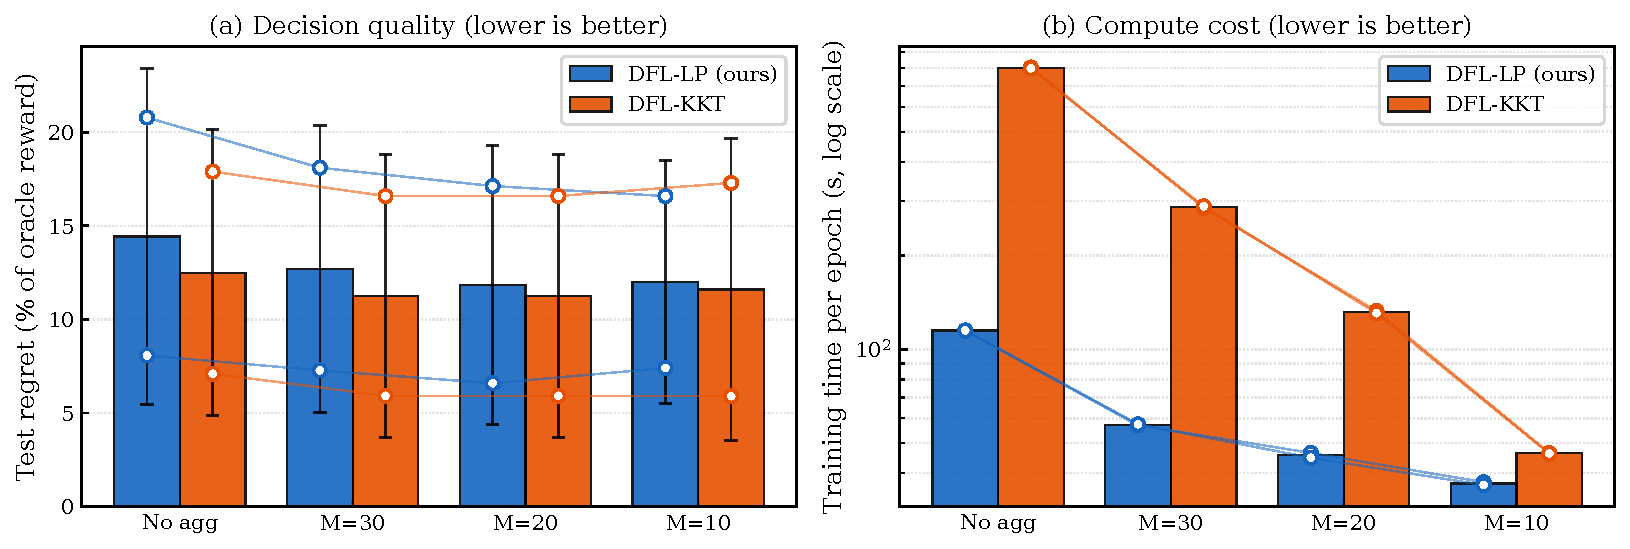
\includegraphics[width=\linewidth]{neurips_2026/figures/elasticity_main.pdf}
  \caption{%
    \textbf{Inventory pricing: state aggregation lowers regret while the LP
    gradient keeps training an order of magnitude cheaper than KKT.}
    Bars show mean over common seeds; hollow markers trace individual seeds
    across the four aggregation levels.
    \emph{(a)} Held-out test regret as a fraction of the oracle reward;
    soft aggregation consistently reduces regret for both gradient variants.
    \emph{(b)} Wall-clock training time per epoch (log scale).
    Without aggregation, DFL-LP is $\sim\!7\times$ faster than DFL-KKT
    ($115$\,s vs.\ $805$\,s per epoch); combining LP with soft aggregation at
    $M{=}10$ yields an additional $\sim\!3\times$ speed-up and matches the
    regret of the full-state KKT baseline.}
  \label{fig:elasticity-main}
\end{figure}

\paragraph{Results.}
\Cref{fig:elasticity-main} summarizes the inventory experiment.
\textbf{(Compute.)} Panel~(b) confirms the $|\gS|$-vs-$|\gS||\gA|$ scaling argument
of~\Cref{tbl:1}: without aggregation, DFL-LP is about $7\times$ faster per
epoch than DFL-KKT ($115$\,s vs.\ $805$\,s). Soft aggregation compounds this
advantage on both sides, shrinking the dominant linear solve from
$|\gS|\times|\gS|$ to $M\times M$; at $M{=}10$ the LP solver completes an
epoch in under $20$\,s.
\textbf{(Quality.)} Panel~(a) shows that soft aggregation also \emph{reduces}
the decision-quality regret of DFL-LP from $14.4\%$ to $11.9\%$ of oracle
(relative reduction $\approx17\%$), and the per-seed traces confirm that this
effect is consistent across both seeds despite the $\sim\!10\%$ spread between
seed-1 and seed-2 realizations. DFL-KKT obtains a slightly lower regret without
aggregation but pays an order-of-magnitude compute premium for it, so the LP
variant with moderate aggregation Pareto-dominates the no-aggregation KKT
baseline on the (time, regret) frontier. These observations support both
claims in~\Cref{sec:agg}: the LP gradient removes the $|\gA|$-dependence in the
linear solve, and state aggregation provides an additional smoothness benefit
on top of that.

\subsection{Cliff Walking}

\subsection{General State MDP}
